%%%%%%%%%%%%%%%%%%%%%%%%%%%%%%%%%%%%%%%%%
% Journal Article
% LaTeX Template
% Version 1.4 (15/5/16)
%
% This template has been downloaded from:
% http://www.LaTeXTemplates.com
%
% Original author:
% Frits Wenneker (http://www.howtotex.com) with extensive modifications by
% Vel (vel@LaTeXTemplates.com)
%
% License:
% CC BY-NC-SA 3.0 (http://creativecommons.org/licenses/by-nc-sa/3.0/)
%
%%%%%%%%%%%%%%%%%%%%%%%%%%%%%%%%%%%%%%%%%

%----------------------------------------------------------------------------------------
%	PACKAGES AND OTHER DOCUMENT CONFIGURATIONS
%----------------------------------------------------------------------------------------

\documentclass[twoside,twocolumn]{article}

\usepackage{blindtext} % Package to generate dummy text throughout this template 

\usepackage[sc]{mathpazo} % Use the Palatino font
\usepackage[T1]{fontenc} % Use 8-bit encoding that has 256 glyphs
\linespread{1.05} % Line spacing - Palatino needs more space between lines
\usepackage{microtype} % Slightly tweak font spacing for aesthetics

\usepackage[english]{babel} % Language hyphenation and typographical rules

\usepackage[hmarginratio=1:1,top=32mm,columnsep=20pt]{geometry} % Document margins
\usepackage[hang, small,labelfont=bf,up,textfont=it,up]{caption} % Custom captions under/above floats in tables or figures
\usepackage{booktabs} % Horizontal rules in tables

\usepackage{lettrine} % The lettrine is the first enlarged letter at the beginning of the text

\usepackage{enumitem} % Customized lists
\setlist[itemize]{noitemsep} % Make itemize lists more compact

\usepackage{abstract} % Allows abstract customization
\renewcommand{\abstractnamefont}{\normalfont\bfseries} % Set the "Abstract" text to bold
\renewcommand{\abstracttextfont}{\normalfont\small\itshape} % Set the abstract itself to small italic text

\usepackage{titlesec} % Allows customization of titles
\renewcommand\thesection{\Roman{section}} % Roman numerals for the sections
\renewcommand\thesubsection{\roman{subsection}} % roman numerals for subsections
\titleformat{\section}[block]{\large\scshape\centering}{\thesection.}{1em}{} % Change the look of the section titles
\titleformat{\subsection}[block]{\large}{\thesubsection.}{1em}{} % Change the look of the section titles

\usepackage{fancyhdr} % Headers and footers
\pagestyle{fancy} % All pages have headers and footers
\fancyhead{} % Blank out the default header
\fancyfoot{} % Blank out the default footer
\fancyhead[C]{5584F $\bullet$ December 2019 $\bullet$ 4F13} % Custom header text
\fancyfoot[RO,LE]{\thepage} % Custom footer text

\usepackage{titling} % Customizing the title section

\usepackage{hyperref} % For hyperlinks in the PDF

\usepackage{graphicx}
\graphicspath{ {images/} }

\newenvironment{reusefigure}[2][htbp]
  {\addtocounter{figure}{-1}%
   \renewcommand{\theHfigure}{dupe-fig}% If you're using hyperref
   \renewcommand{\thefigure}{\ref{#2}}% Figure counter is \ref
   \renewcommand{\addcontentsline}[3]{}% Avoid placing figure in LoF
   \begin{figure}[#1]}
  {\end{figure}}
\usepackage{wrapfig}
\usepackage{amsmath}
\usepackage{xcolor}
\usepackage{listings}
\usepackage{subcaption}
\usepackage{pdfpages}
\usepackage{array,multirow,graphicx}
\lstset{
  basicstyle=\ttfamily,
  columns=fullflexible,
  frame=single,
  breaklines=true,
  postbreak=\mbox{\textcolor{red}{$\hookrightarrow$}\space},
}

%----------------------------------------------------------------------------------------
%	TITLE SECTION
%----------------------------------------------------------------------------------------

\setlength{\droptitle}{-4\baselineskip} % Move the title up

\pretitle{\begin{center}\Huge\bfseries} % Article title formatting
\posttitle{\end{center}} % Article title closing formatting
\title{4F13 - Coursework Three - Latent Dirichlet Allocation } % Article title
\author{%
\\
\textsc{Candidate Number: 5584F} \\
\normalsize Word count: 1000 \\
}
\date{\today} % Leave empty to omit a date
\renewcommand{\maketitlehookd}{%
}

%----------------------------------------------------------------------------------------

\begin{document}
\onecolumn
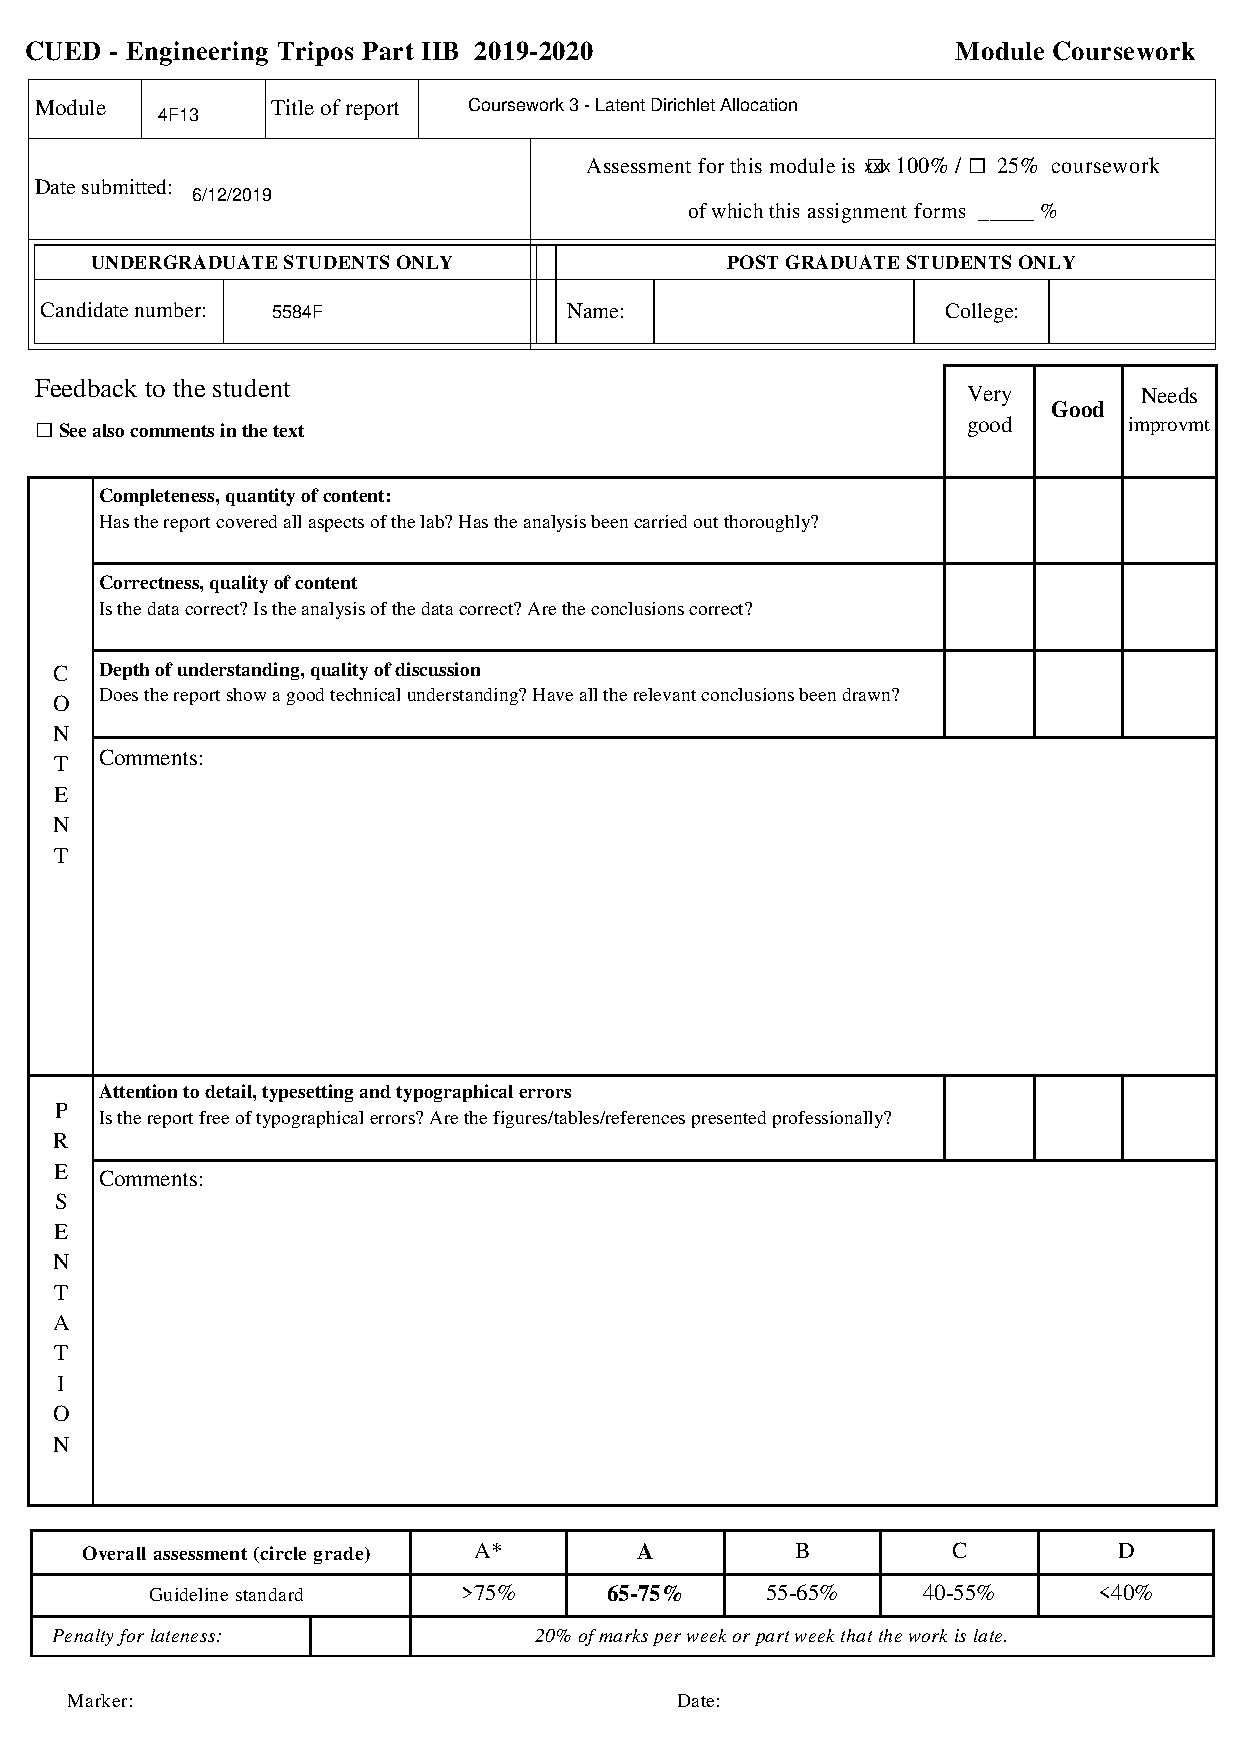
\includepdf[pages={1}]{Coversheet.pdf}
\twocolumn
% Print the title
\maketitle

%----------------------------------------------------------------------------------------
%	ARTICLE CONTENTS
%----------------------------------------------------------------------------------------



\section{a}
Using word count data different models for the probability of each word appearing can be created. The simplest model is to perform maximum likelihood optimisation using occurrences seen in training documents. As in equation \ref{eq:ml} this requires computing the total count of each word and then renormalising to generate a multinomial distribution. Figure \ref{fig:a_1} shows the 20 most common words and their probabilities under this model. 

\begin{equation}
p_m^{(ML)} = \frac{c_m}{\sum_lc_l}= \frac{c_m}{N}\\
\label{eq:ml}
\end{equation}

This distribution can be used to calculate the probability of a document given the model. In this simple model each document follows the same distribution, irrespective of their document class. To maximise the log probability the test document should contain only the most probably word from training as independence is assumed between words, a document with only one word would maximise this with log probability = log($p_{max}$). The minimum probability occurs when the test document contains at least one new word so has log probability -$\infty$. The implications of this are that new words will break document testing due to a zero probability and atypical sequences of the same word are individually more likely then typical sequences observed in a real document. Considering sequence probabilities and combination factors into the model could solve the latter problem.


\begin{figure}[h]
  \centering
    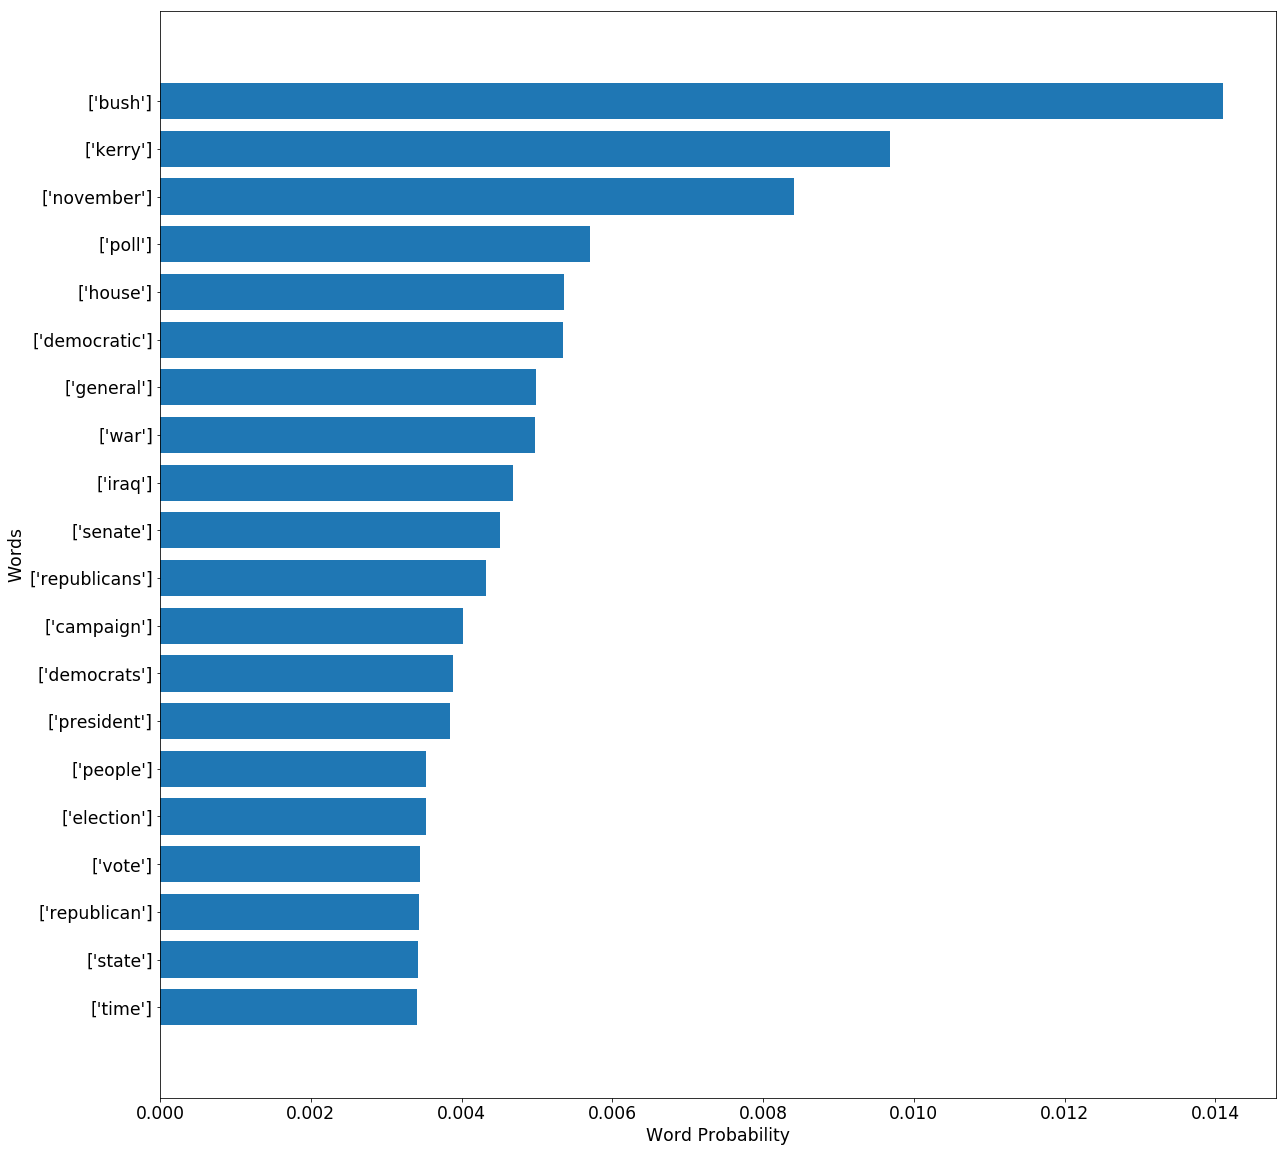
\includegraphics[width=\linewidth]{a_1}
  \caption{Most probable words under simple model}
  \label{fig:a_1}
\end{figure}
%-----------------------------------
\section{b}
A better method of model generation uses a prior distribution and inference to update the model after observations. For this a symmetric Dirichlet model with parameter $\alpha$ is used. Equations \ref{eq:dir} shows the prior and the posterior update for a K dimensional distribution, re-normalisation is essential after the update.

\begin{equation}
\begin{split}
Dir(K, \boldsymbol{\alpha}) \rightarrow Dir(K,c_1+\alpha_1,....., c_K + \alpha_K )
\end{split}
\label{eq:dir}
\end{equation}

When using this model to predict word probabilities in test data the categorical word probabilities are first drawn from the Dirichlet distribution. After this both models follow equation \ref{eq:dir2} to calculate the probability of the document given the model.

\begin{equation}
\begin{split}
p(\textbf{W}_{d}|\boldsymbol{\beta})= \prod_{n=1}^N  p(W_{nd}|\boldsymbol{\beta})
\end{split}
\label{eq:dir2}
\end{equation}

When $\alpha$ = 1 the prior is a uniform distribution, with higher values giving more certainty that uniformity is desired as $\alpha$ can be though of as psudo-counts. This prior leads to unseen words in training having a non-zero probability associated with them. Figure \ref{fig:b_1} shows the probabilities of each word for various $\alpha$'s. Increasing $\alpha$ has the effect of making all probabilities in $\boldsymbol{\beta}$ more equal. Increased by the right amount it can ensure unseen words have a reasonable probability and common word probabilities aren't inflated by their usually high training presence. These both reduce overfitting. To further generalise the model to infinite new words a Dirichlet process could be used.

\begin{figure}[h]
  \centering
    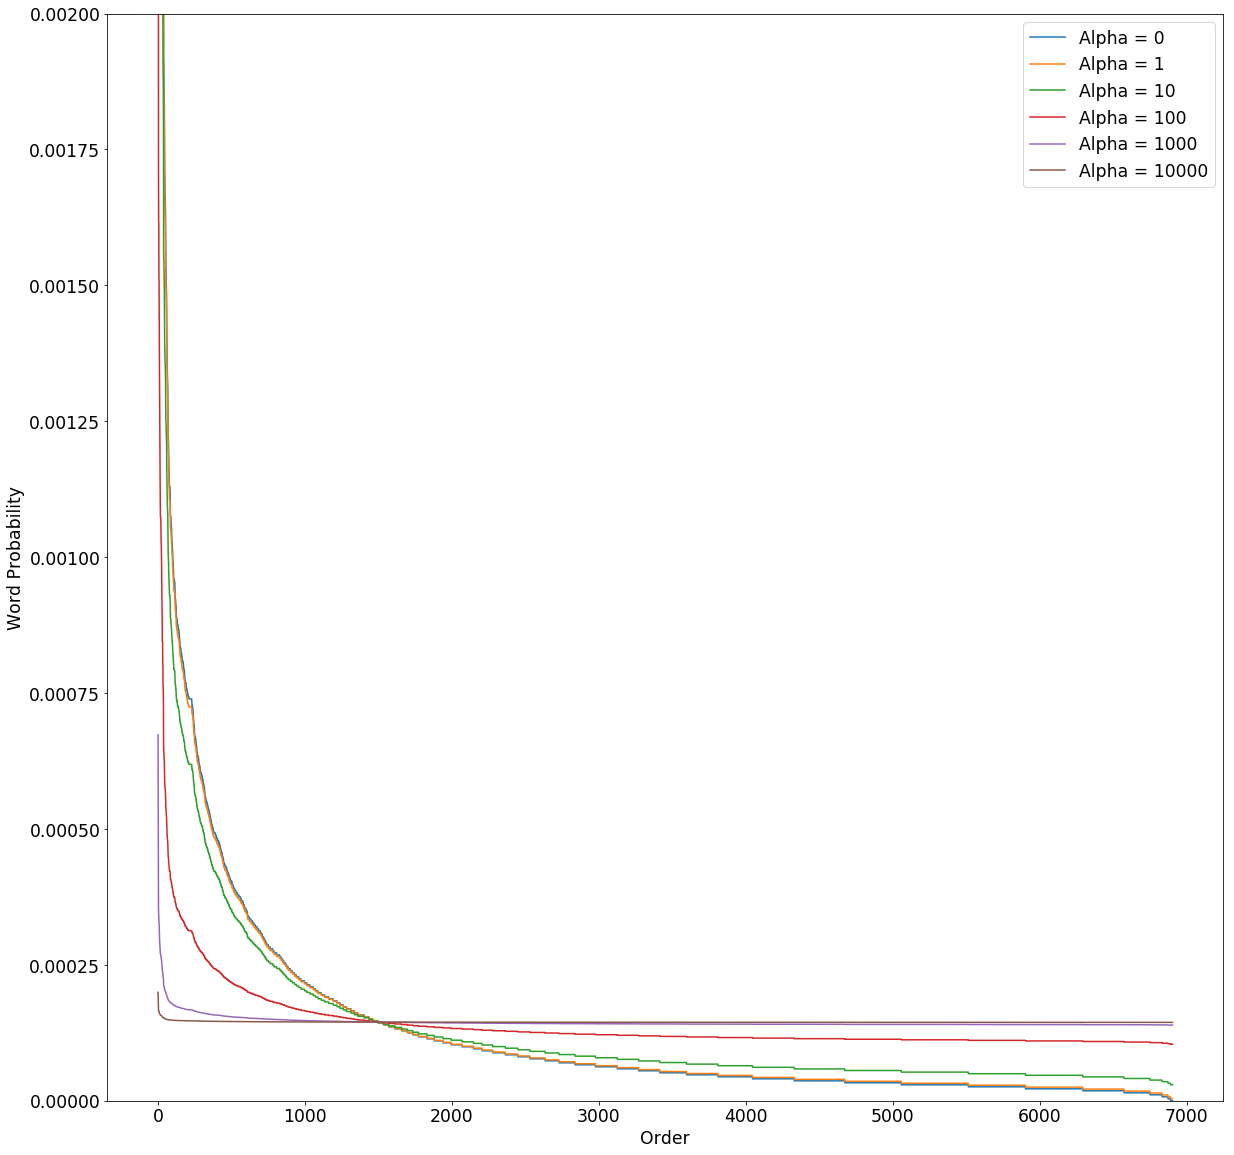
\includegraphics[width=\linewidth]{b_1}
  \caption{Effect of changing $\alpha$ in prior, zoomed into lower probabilities}
  \label{fig:b_1}
\end{figure}

%------------------------------------------------
\section{c}

\begin{equation}
\begin{split}
p(\textbf{W}_{d}|\boldsymbol{\beta})=\frac{N!}{\prod_{u=1}^Uc_u!} \prod_{n=1}^N  p(W_{nd}|\boldsymbol{\beta})
\end{split}
\label{eq:dir3}
\end{equation}

The probabilities of a test document under the Baysian model can be calculated as in equation \ref{eq:dir2}. This uses a categorical distribution function. However, if the combinations of word position within a document are considered as in equation \ref{eq:dir3} you can predict from a multinomial distribution. Table \ref{table:c1} shows some of these probabilities. When using a categorical distribution atypical documents such ones with one word have a high probability compared to typical documents. However, if we assume that all documents being compared are typical with similar word proportions then this effect can be ignored and the word counts alone can be used for simplicity.

\begin{table}[h]
\centering
\begin{tabular}{ c | c | c }
$\alpha$& categorical&multinomial\\ 

\midrule
0& -3691.5.6&-1691.1\\
1&-3688.6&-1688.2\\
5&-3640.7&-1640.3\\
10&-3592.1&-1591.8 \\
100&-3199.1&-1198.6\\
\end{tabular}
\caption{log probabilities of test document 2001}
\label{table:c1}
\end{table}


The per-word perplexity can be calculated using equation \ref{eq:pwp}. Perplexity is a good way of evaluation language models as a small value  relates to high probability under the model. Figure \ref{fig:c_1} shows the perplexity for document 2001 and test average. A minima is observed in each case which corresponds to the best mix between learning from training and incorporating new words into the model. Per-word perplexities differ between documents as each document has different word counts and probabilities under the trained model. 

\begin{equation}
Perplexity = exp ( - \frac{\sum_{d=1}^D log (p(\textbf{W}_{d}|\boldsymbol{\beta}))}{\sum_{l\; in \;test}c_l})
\label{eq:pwp}
\end{equation}

\begin{figure}[h]
  \centering
    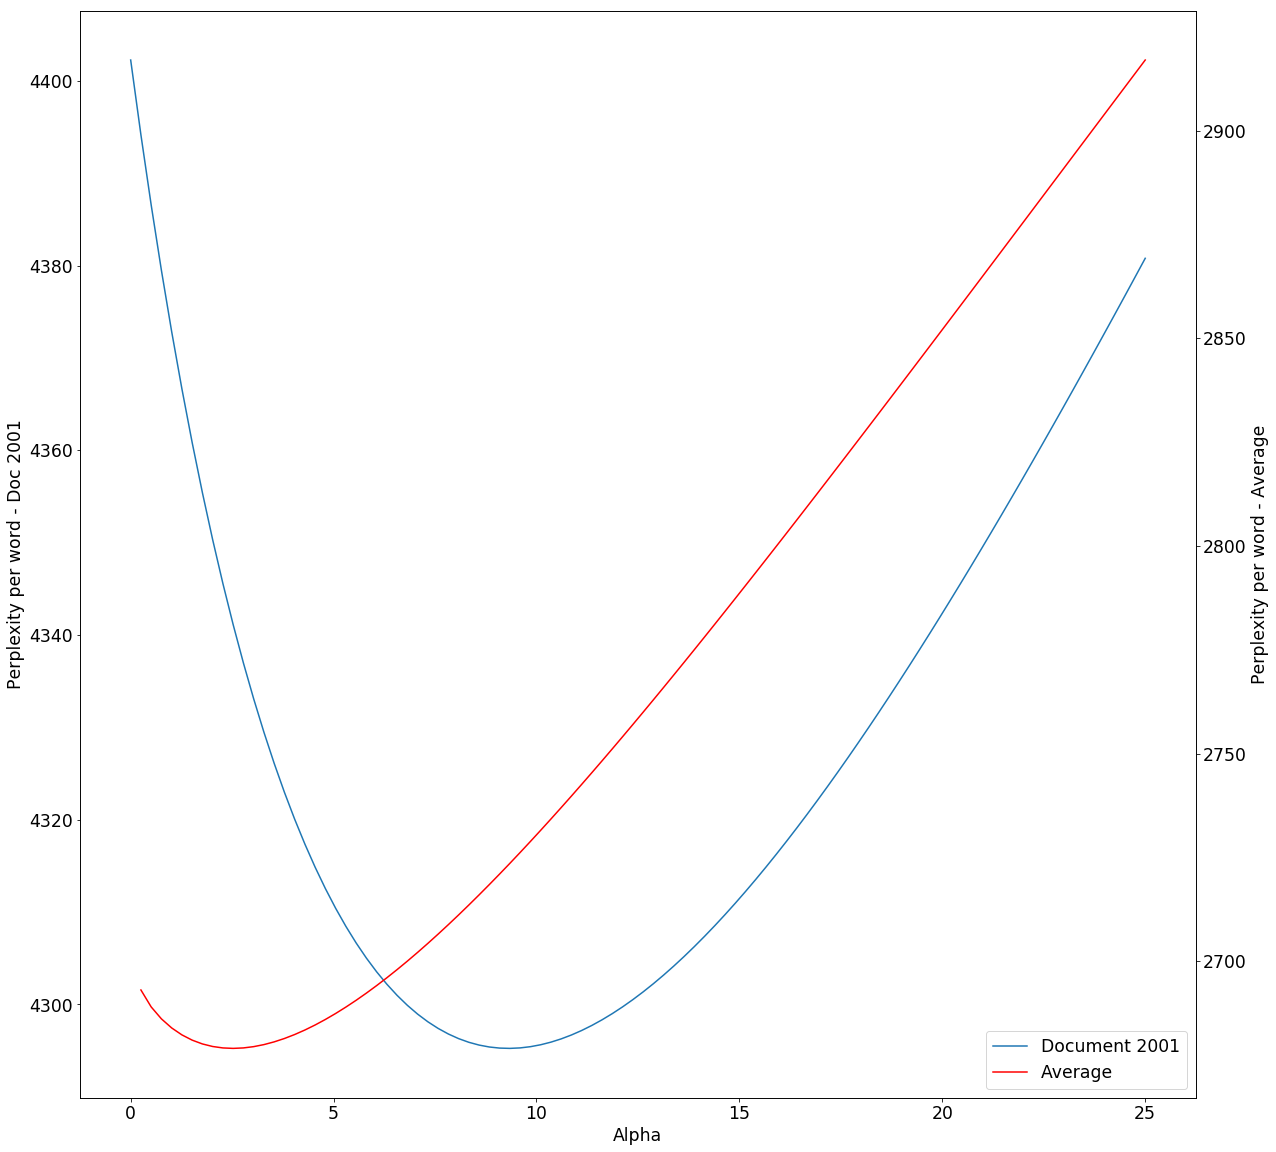
\includegraphics[width=\linewidth]{c_1}
  \caption{Test Perplexities for various $\alpha$ values and test documents}
  \label{fig:c_1}
\end{figure}
The per-word perplexity under a uniform multinomial distribution for document d is shown in equation \ref{eq:uni}, for document 2001 this has a value of 6906. Which is higher then the Baysian model as expected.
\begin{equation}
Perplexity = exp ( - \frac{log \frac{1}{N}^{N_d}}{N_d}  )
\label{eq:uni}
\end{equation}
%------------------------------------------------
\section{d}
The model can be further improved by introducing different topics and having each document a member of one topic. The effect of this when testing is to first assign the document a categorical distribution across words $\boldsymbol{\beta_k}$. This is done using another Dirichlet distribution over all categories and the probability a document belongs in group k ($\boldsymbol{\theta}$). The Dirichlet parameters used were 10 for document mixing and 0.1 for word distributions.
\newline
Gibbs sampling is required when calculating these extra probabilities. This is due to calculating the exact distribution being intractable. Within the iterations each variable is being sampled to collapse the model to a simpler categorical distribution. In this process documents are progressive updated with a new class until convergence. Figure \ref{fig:d_1} shows the convergence in a Baysian mixture model with 20 groups. Convergence is achieved as each line plateaus so has constant mean in addition to constant consisted variance as shown in figure \ref{fig:d_2}. The largest group converges the slowest in 25 iterations. To determine the stationary distribution more carefully additional Gibbs iterations could be performed and longer averages taken. Taking account of the auto correlation between samples in this average would further improve certainty convergence as been achieved.

\begin{figure}[h]
  \centering
    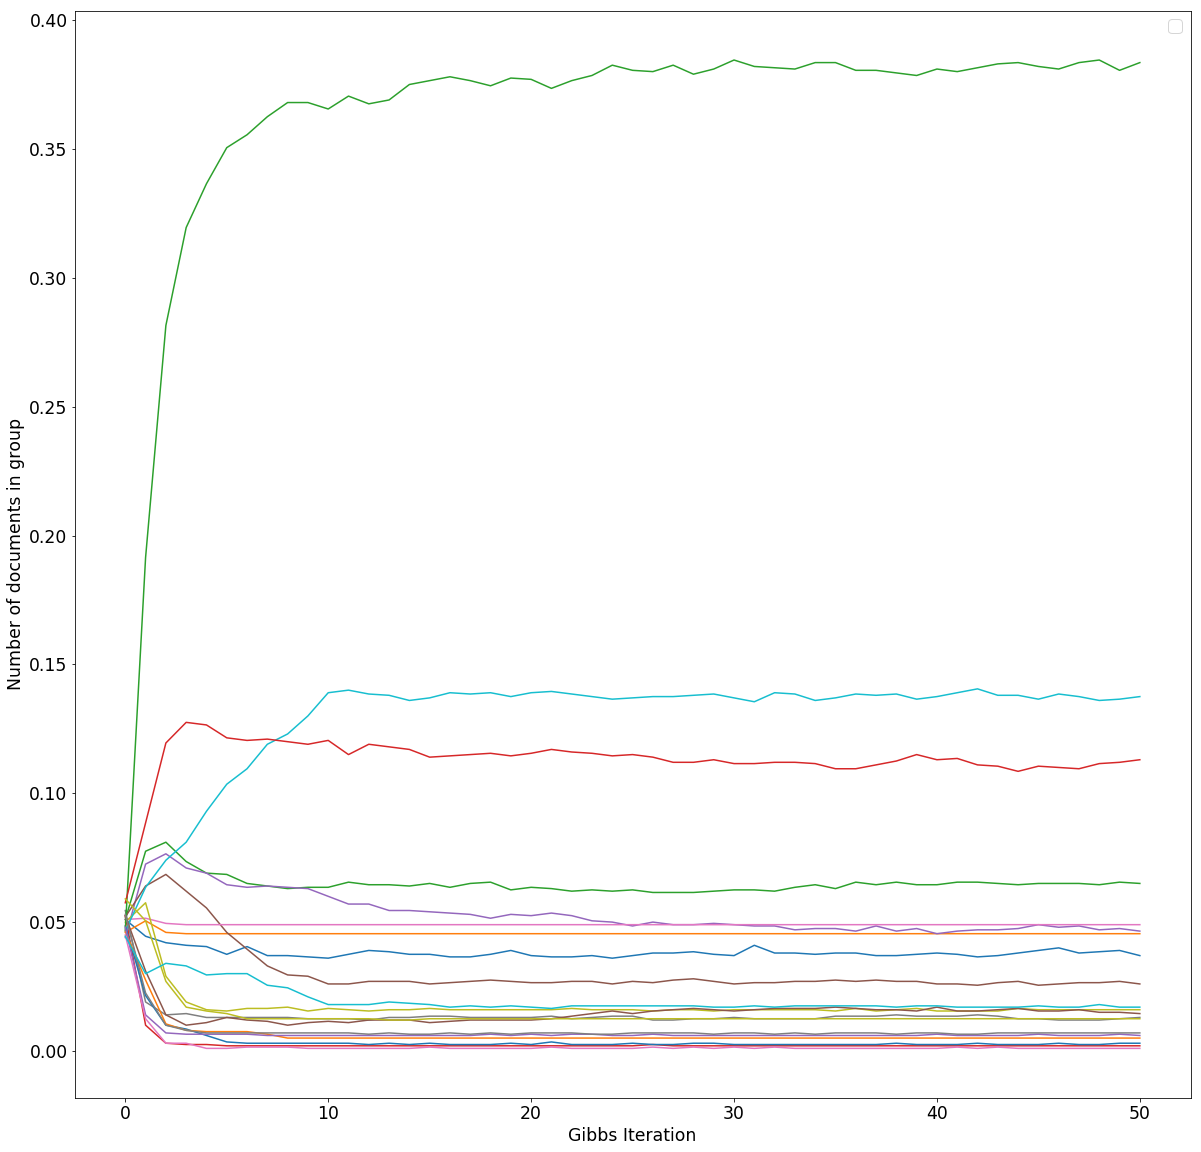
\includegraphics[width=\linewidth]{d_1}
  \caption{Document mixing proportions vs Gibbs sample iteration in Baysian mixture model}
  \label{fig:d_1}
\end{figure}

\begin{figure}[h]
  \centering
    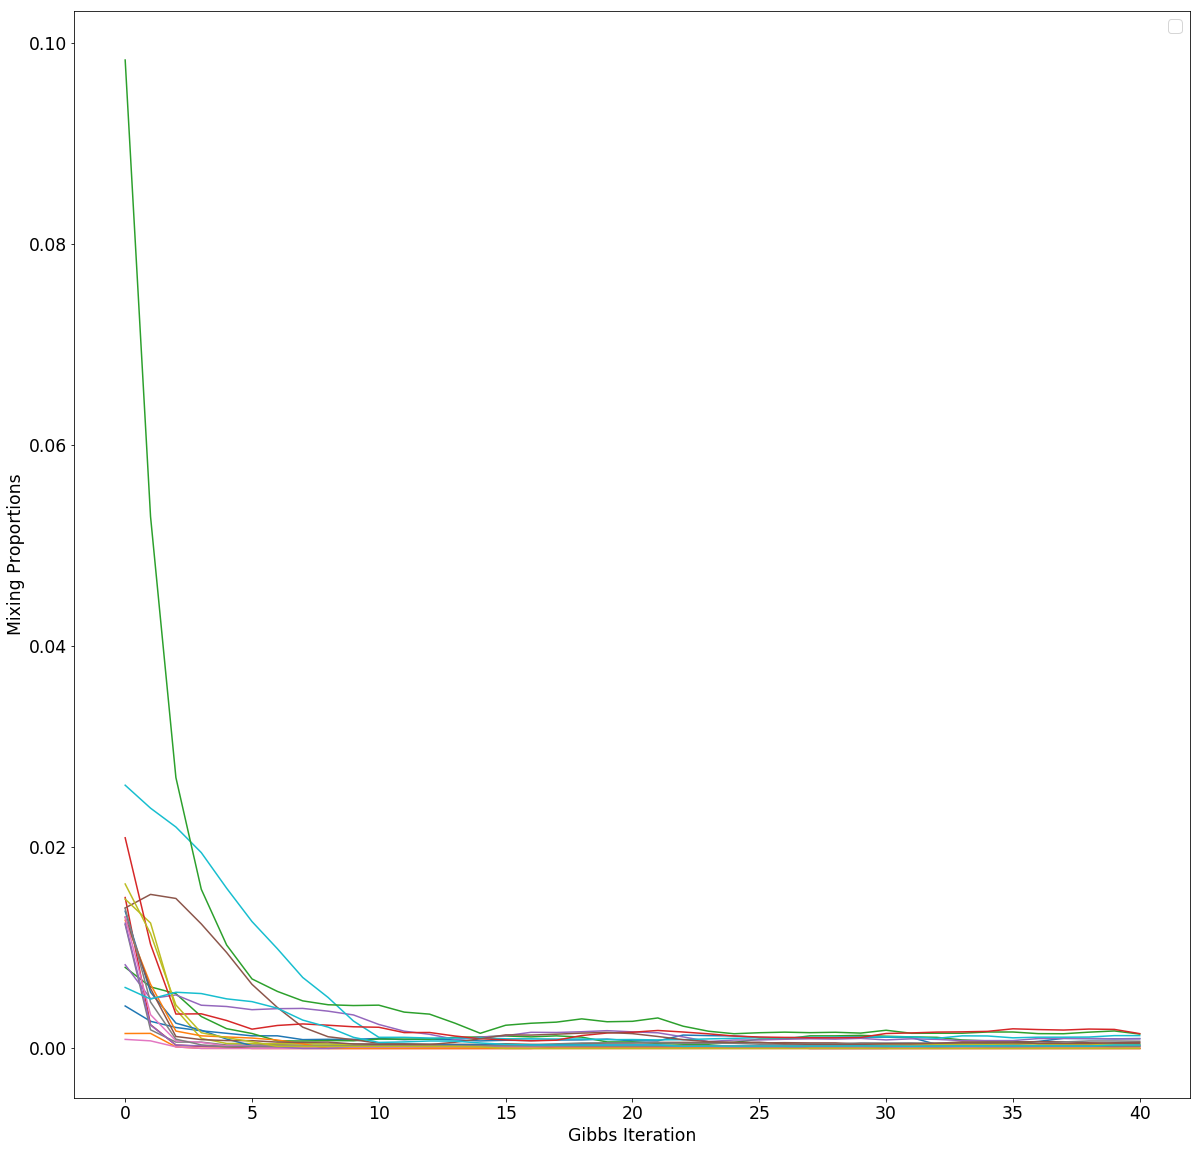
\includegraphics[width=\linewidth]{d_2}
  \caption{Standard deviation of mixing proportions for next 10 iterations in BMM, }
  \label{fig:d_2}
\end{figure}

%------------------------------------------------------
\section{e}
In latent Dirichlet allocation documents individual words within a document can be assigned different topics. This is done by having a mixing proportion across topics for each document, with each word within the document having its topic and categorical word distribution drawn from the document mixture. This change is advantageous as it allows for multi-topic documents to be accurately modelled. Gibbs sampling is used once again to make the problem tractable. Figure \ref{fig:e_1} shows the convergence for the mixing proportion of words. Convergence is slower then in a BMM which is expected as the number of words is far larger then number of documents. After around 40 iterations the means and standard deviations in figure \ref{fig:e_2} appear to have settled. However, some groups such as orange seem to still be changing after 50 iterations. For this reason I would say 50 sweeps is inadequate to reach a stationary distribution. 

\begin{figure}[h]
  \centering
    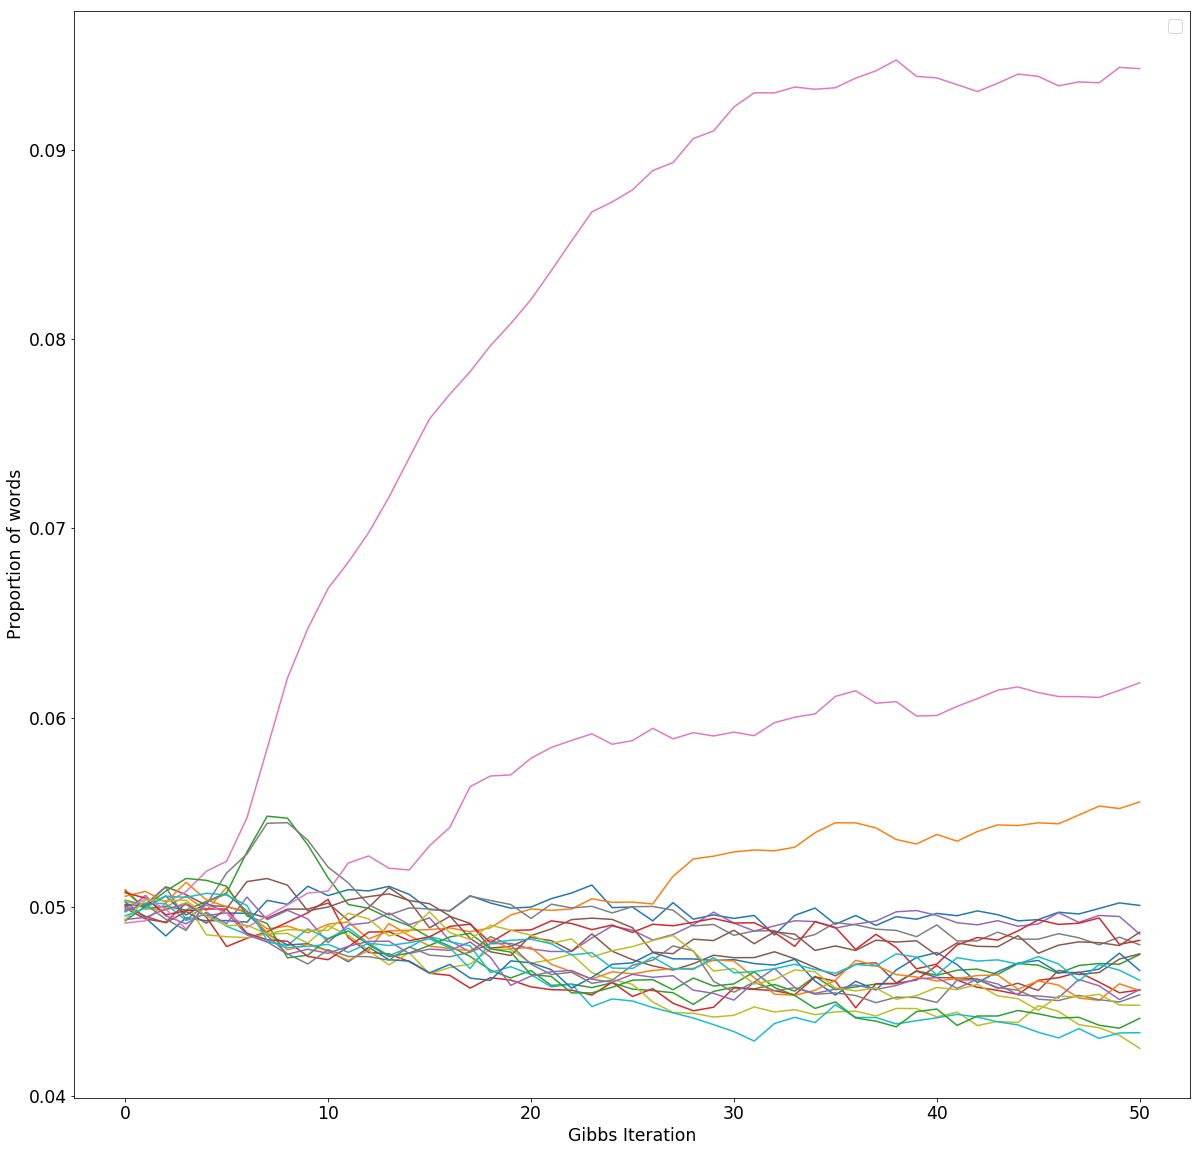
\includegraphics[width=\linewidth]{e_1}
  \caption{Word mixing proportions vs Gibbs sample iteration in LDA model}
  \label{fig:e_1}
\end{figure}

\begin{figure}[h]
  \centering
    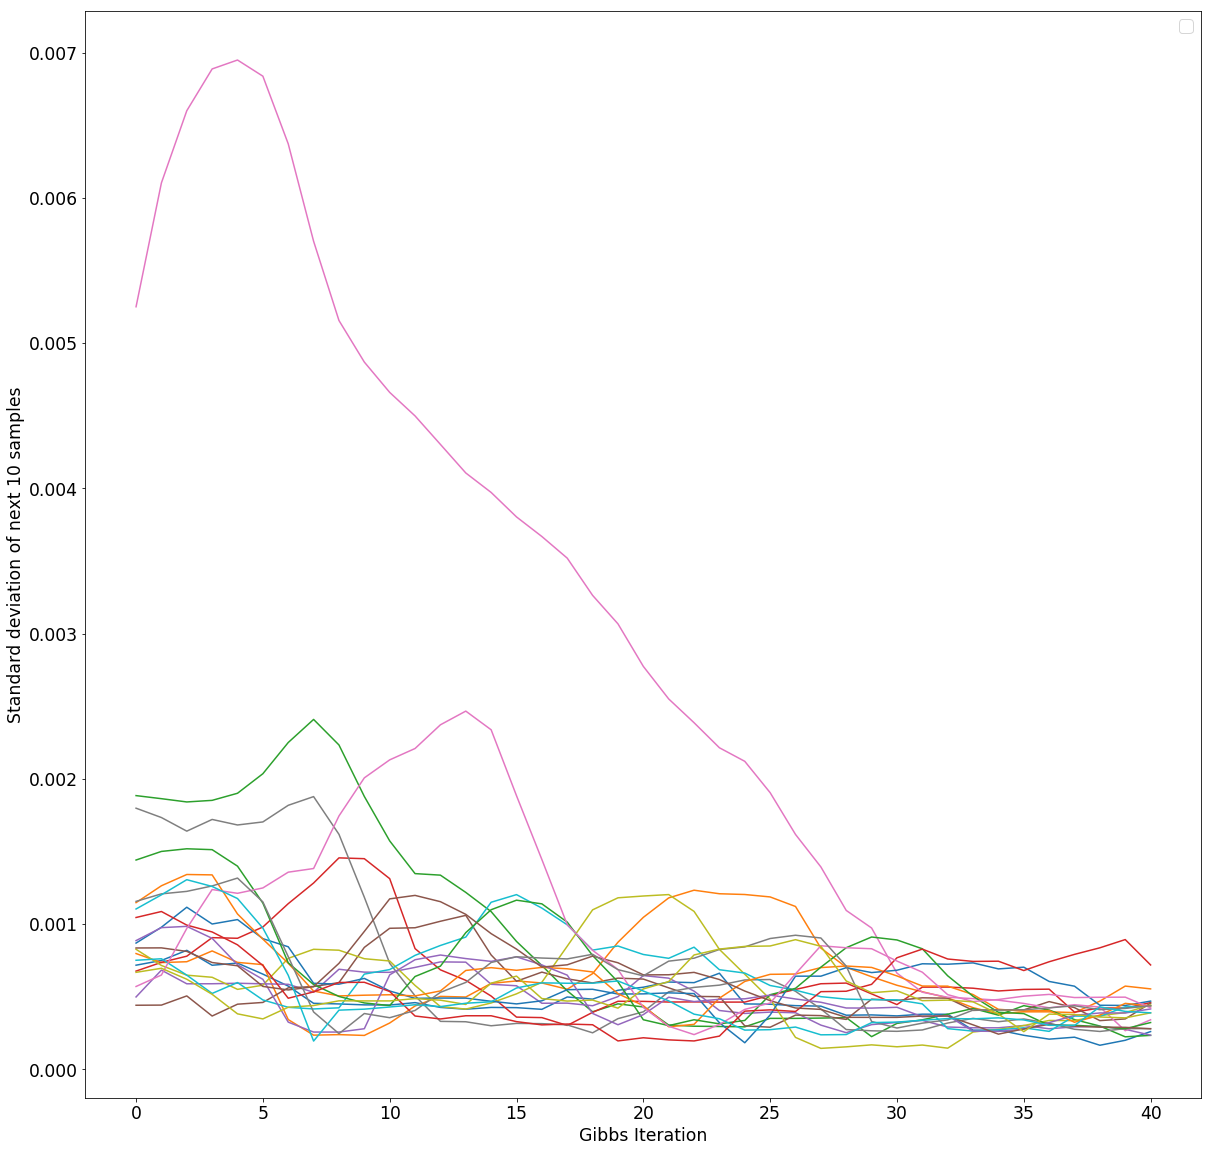
\includegraphics[width=\linewidth]{e_2}
  \caption{Standard deviation of mixing proportions for next 10 iterations in LDA}
  \label{fig:e_2}
\end{figure}

The per-word perplexity can once again be calculated, across all the test docments this has a value of 2071.7. Comparing this to BMM at 2127.8 and the simpler model in figure \ref{fig:c_1} with minima at 2675, its clear that the LDA model creates the best generalised model for a variety of test documents.

\begin{figure}[h]
  \centering
    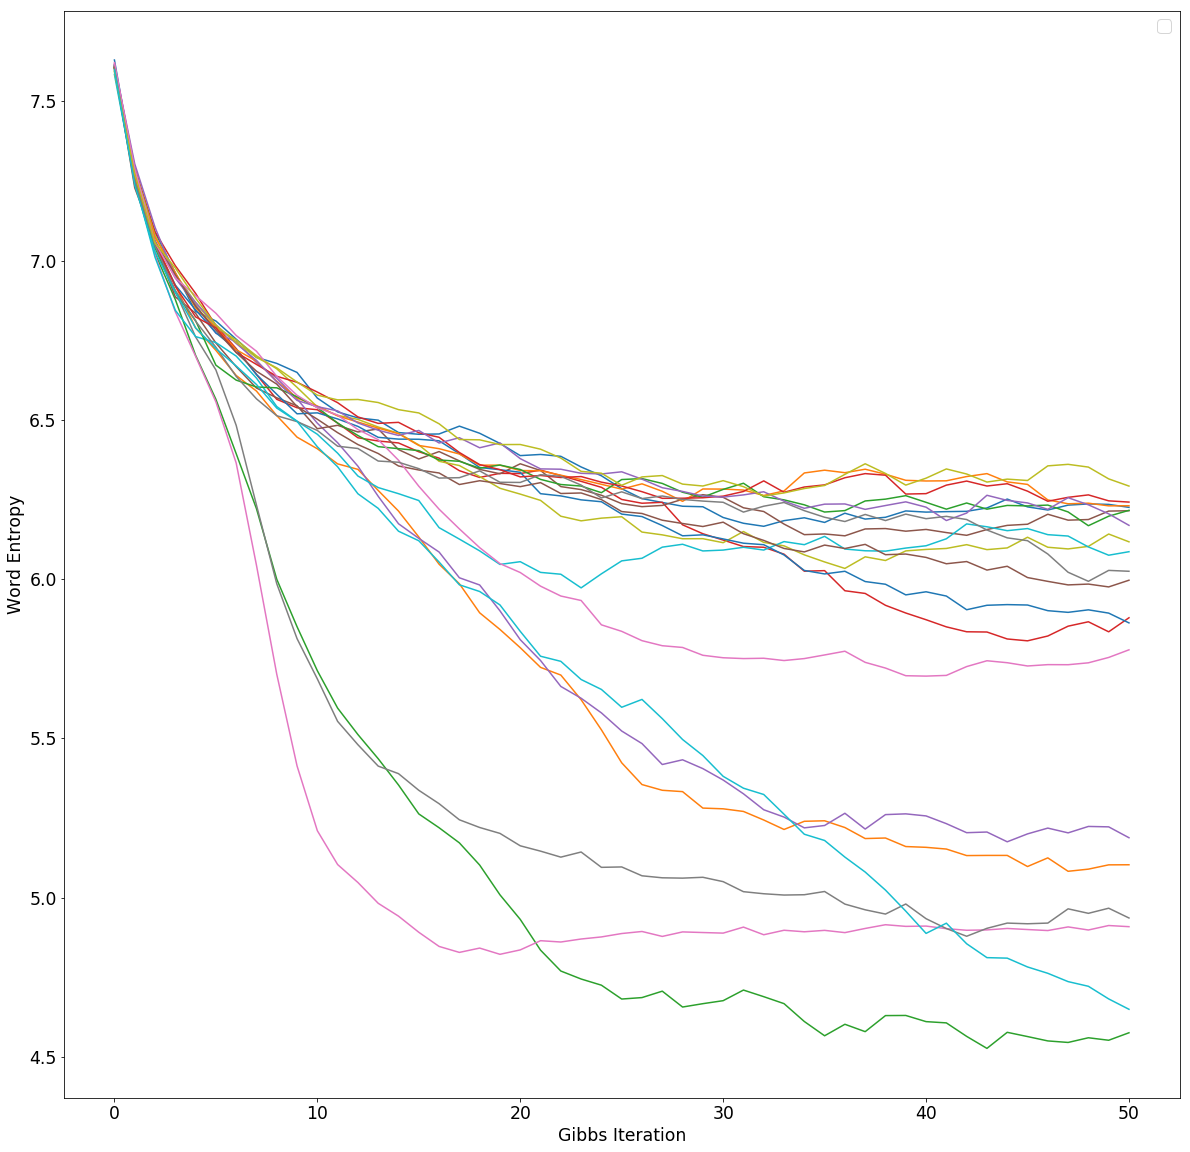
\includegraphics[width=\linewidth]{e_3}
  \caption{Word entropies within a topic}
  \label{fig:e_3}
\end{figure}

The word entropies can be calculated for each Gibbs iteration, this uses the number of unique words assigned to each topic. Figure \ref{fig:e_3} shows this entropy across iterations. The units are nats.  Initially all groups have the same entropy as groups start off randomly assigned. As iteration number increases the entropies drop, this is as expected as this means that the groups are approaching a distinct distribution that is not uniform. A decrease in entropy can be thought of as each topic only containing the minimum words required to model that subject.

\section{Appendix}
\subsection{a}
\begin{lstlisting}[language=python]
for i in range(N_1):
    counts[A[i,1]-1]+=A[i,2]
mlm = counts/N_w
\end{lstlisting}

\subsection{b}
\begin{lstlisting}[language=python]
alpha=10
dp = (counts + alpha)/(N_w+W*alpha)
sorted_word(dp,V,M)
\end{lstlisting}


\subsection{c}
\begin{lstlisting}[language=python]
def log_prob(model, document):
    c = document[:,2]
    log_prob = np.dot(c, np.log(model[document[:,1]-1])) 
    return log_prob

def get_per(model,document,combi=False):
    if combi == True:
        lp = combi_log_prob(model,document)
    else:
        lp = log_prob(model,document)
    n = np.sum(document[:,2])
    return np.exp (-lp/n)
\end{lstlisting}


\subsection{d}
\begin{lstlisting}[language=python]
mixing_prop[iter+1, :] = sk_docs[:,0]
\end{lstlisting}

\subsection{e}
\begin{lstlisting}[language=python]
mixing_prop = np.zeros((num_gibbs_iters+ 1, K))
    word_entropy = np.zeros(mixing_prop.shape)
    mixing_prop[0, :] = sk
    for k in range(K):
        word_entropy[0, k] = entropy(swk[:, k])

\end{lstlisting}

%------------------------------------------------
\end{document}
